\Chapter{Felhasznált technológiák és fejlesztői környezetek}

\Section{Backend}

A backend a web fejlesztés szerver oldala amit nem lát a felhasználó. Itt szokott történni az adatbázissal való kommunikálás. Itt történnek az authentikációk(hitelesítések) és az authorizációk(engedélyezések). Nagyon sok féle backend technológia létezik mint például: PHP, Python, Node.js, Java. Mint már említettem én a Javat fogom használni a fejlesztések során.

\subsection{Java}

A Java egy objektum orientált programozási nyelv, amit James Gosling fejlesztett a 90’-es években Sun Microsystemsnél. Eredetileg televíziózásra készült, de azokban az időkben túlságosan fejlett volt hozzá.

Java célja a hordozhatóság ami azt jelenti, hogy a Java-ban írt programoknak hasonlóan kell futnia bármely operációs rendszeren. Java nyelvi kódot először bájtkódra fordítják ami hasonló a gépi kódhoz, de virtuális gép általi végrehajtásra készülnek. Vannak mikro vezérlők mik képesek a Java bájtkódját hardverben futtatni.

Java a Szintaxisát a C és C++ nyelvből örökölte, még a C++ egyesíti a strukturált, általános és objektumorientált programozás szintaxisát addig a Java csak Objektumo-
rientált nyelvnek készült. Java nem támogatja az operátok túlterhelést vagy a többszö-
rös öröklődést (interfészek esetében lehetséges).

Java jelenlegi tulajdonosa az Oracle Corporation 2010-óta hogy felvásárolta a Sun Microsystems-t.

Java az egyik legelterjedtebb programozási nyelv, mivel mindegyik operációs rend-
szerre tudunk vele alkalmazást fejleszteni, és könnyen tanulható. Nagyon felhasználó barát.\cite{Java}

\subsection{Spring Boot}

A Spring Boot Spring-keretrendszerre épülő bővítmény a Spring pedig egy Java alapú webalkalmazás-keretrendszer, ami nyílt forráskódú. A Spring Testreszabott Webal-
kalmazások létrehozásához tökéletes ami teljesen konfigurálható az előre elkészített kódterekkel és kódtárakkal. Spring Bottal különálló Spring alkalmazásokat hozhatunk létre amit azonnal futtathatunk.

Spring Boot használata nagyon egyszerű, jó minőségű alkalmazásokat lehet benne fejleszteni kevesebb fejlesztési idő alatt. Beépített http-kiszolgálókat tartalmaz, mint a Tomcat és Jerry.

Spring Boot tartalmaz egy Maven-hez tartozó (POM.XML) fájlt, amiben spring-boot-dependencies-eket tudunk megadni, mint például:

\begin{itemize}
\item spring-boot-starter-web
\item spring-boot-starter-data-jpa
\item spring-boot-starter-test
\end{itemize}

A POM.XML egy konfigurációs fájl ként is használható

Spring initializr: Segítségével könnyedén „összekattintgathatjuk” a projektünk alap-
ját, megadhatunk függőségeket, megadhatjuk, hogy milyen programozási nyelven sze-
retnénk elkészíteni, a projekt nevét. \cite{SpringBoot}

\Section{Adatbázis}
Az adatbázis nem más, mint elektronikusan tárolt adatok, amihez hozzá lehet férni.


\subsection{PostgreSQL}

Nyílt forráskódú relációs adatbázis kezelő rendszer ami az egyik legrégebbi relációs adatbázis nem mellesleg ingyenes. Relációs adatbázisok relációs modellen alapulnak. A relációs modell az adatokat egy vagy több sorból és oszlopból álló táblázatba(relációba) rendezi és minden sorhoz rendel egy egyedi kulcsot.

A PostgreSQL Kaliforniai egyetem Ingres projektjéből fejlődött. Az összes operációs rendszerrel kompatibilis. Támogatja a relációs és a nem relációs lekérdezéseket is így JSON vagy SQL alapú útvonal-kifejezésekkel is elérhetőek az adatok.  Mind ezek miatt az egyik leghasználtabb Adatbázis-motor.\cite{PostgreSQL}

\begin{figure}[h]
\centering
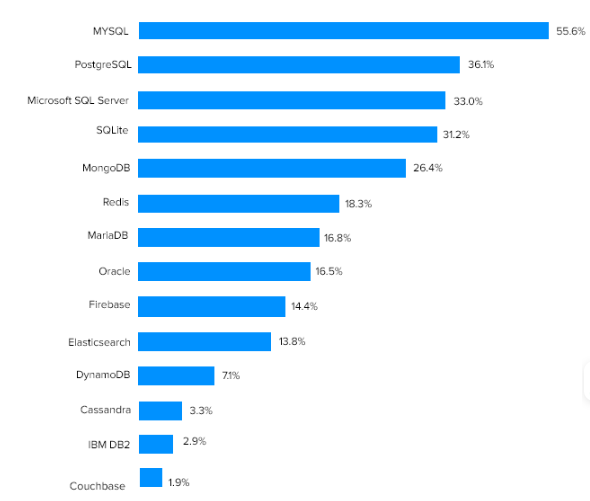
\includegraphics[scale=0.6]{images/top14_database.png}
\caption{14 leghasználtabb adatbázis.\cite{databases}}
\label{fig:Adatbázisok}
\end{figure}
\newpage

\Section{Front-end}

A frontend a szoftver megjelenítési rétege. A weboldalnak azon réteg amit a felhasználó is lát és interakcióba tud vele lépni. Legfontosabb része a HTML(Hypertext Markup Language) ez adja meg a Weboldal kinézetének a vázát és hozzá csatlakozik a CSS(Cas-cading Style Sheets) ami segítségével egyedi megjelenést biztosíthatunk a weboldalunk-
nak. Több fajta framework létezik Front-end fejlesztésre mint például:

\begin{itemize}
\item React
\item Angular
\item Vue.js
\end{itemize}


\subsection{Angular}

Az Angular egy TypeScript-alapú nyílt forráskódú webalkamazás-keretrendszer. 2016-ban jelent meg az első verzió.

Egyben tartalmazza TypeScript osztályt HTML-sablont stílusokkal. HTML sablon lehetővé teszi dinamikus értékek beszúrását mint például szöveg. Tartalmaz komponen-
seket ezek NgModulokba vannak rendezve. Minden alkalmazásnak van egy úgynevezett gyökérmodulja aminek a neve általában az AppModule, amely a bootstrap mechaniz-
must biztosítja, amely elindítja az alkalmazást. Ngmodulok is importálhatnak más Ngmodulokat, például az útválasztó szolgáltatás használatához a Router NgModul-t.  Minden Angular alkalmazásnak van egy gyökérkomponense, ami összekapcsolja a komponens hierarchiát. Mindegyik komponenshez tartozik egy HTML-sablon, ami se-
gítségével megjeleníthető a tartalom. Tartalmaz egy services osztályt is ezt akkor használjuk ha van olyan adat vagy logika, amelyek nem kapcsolódnak, de meg szeret-
nénk osztani a komponensek között.\cite{Angular}

\Section{Fejlesztői környezetek és fejlesztéshez használt p-rogramok}

\subsection{Intelij IDEA}

Egy integrált fejlesztői környezet amit a JetBrains fejlesztett ki. Ebben az IDEA-ban Java, Kotlin Groovy és más JVM alapú nyelveken írt szoftvereket lehet fejleszteni. Az integrált fejlesztői környezet(IDE)  egy olyan  szoftveralkamazás, amely átfogó lehetősé-
geket biztosít a számítógép programozóknak a szofverfejlesztéshez . Az IDE általában legalább egy forráskód-szerkesztőből ,építési autómatizálási eszközökből és egy hiba-
keresőből áll . Egyes IDE-k, például a NetBeans és az Eclipse tartalmazzák a szükséges fordított , értelmezőt vagy mindkettőt; mások, például a SharpDevelop és a Lazuras nem.\cite{Intelij}\cite{Intelij2}
\newpage

\begin{figure}[h]
\centering
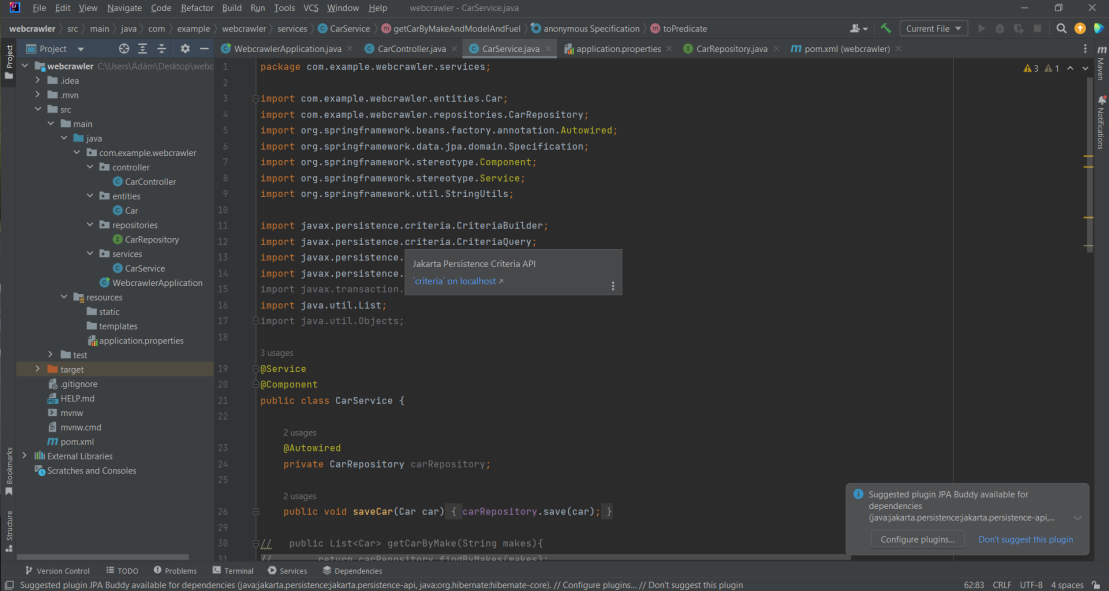
\includegraphics[scale=1]{images/Intelij.png}
\caption{Intelij IDEA.}
\label{fig:Intelij}
\end{figure}

\subsection{Visual Studio Code}

VS Code egy forráskód szerkesztő amit a Microsoft fejlesztett ki 2015-ben csak Win-
dows Linux és MacOS operációs rendszereken elérhető. Nagyon sok programozási nyelv-
vel lehet használni mint például:

\begin{itemize}
\item JavaScipt
\item Go
\item Node.js
\item C++
\item Phyton
\end{itemize}

Rengeteg kiegészítővel lehet bővíteni a fejlesztő környezetet ami könnyebbé és átlát-
hatóbbá teszi  fejlesztést, ezért esett nekem a választás erre a környezetre a frontend fejlesztéséhez.\cite{VSCode}

\begin{figure}[h]
\centering
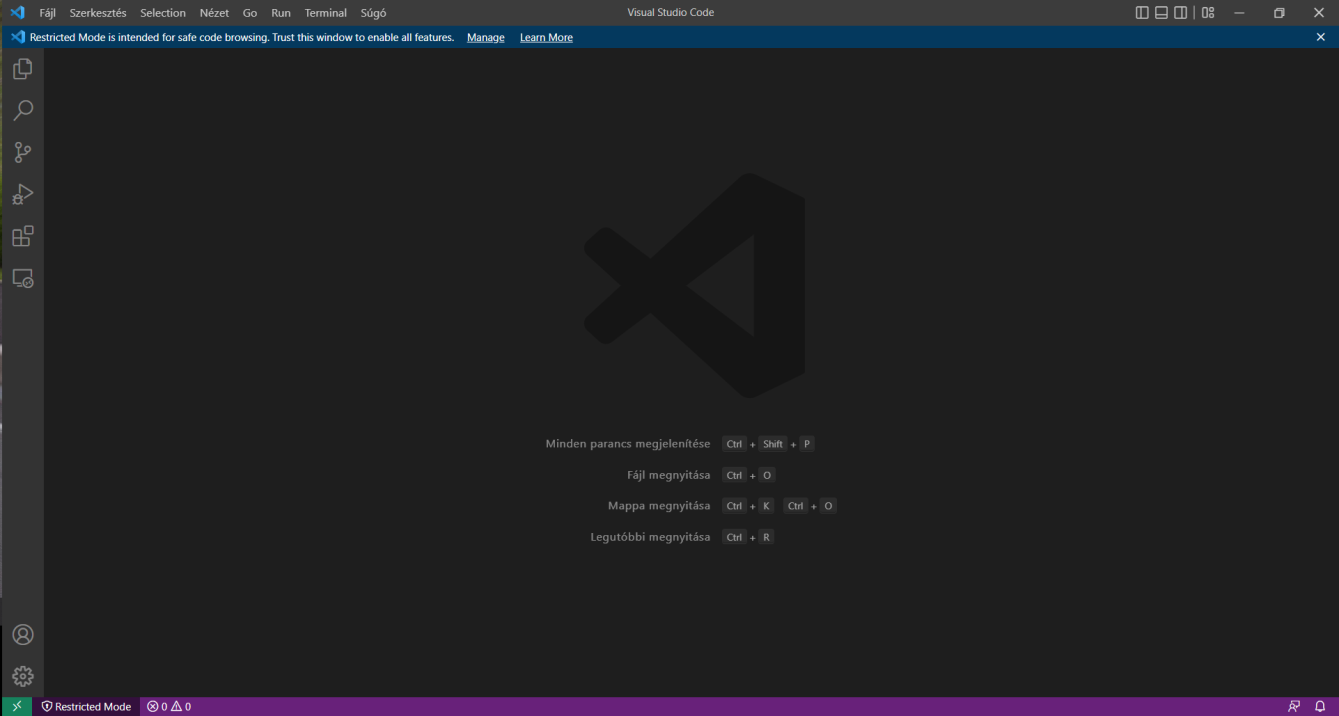
\includegraphics[scale=0.6]{images/VSCode.png}
\caption{Visula Studio Cods.}
\label{fig:VSCode}
\end{figure}
\newpage

\subsection{Postman}

A Postman\cite{Postman} API-k létrehozására és használatára, tesztelésére létrehozott plattform. Használatával egyszerűbben és gyorsabban hozhatunk létre jobb minőségű API-kat. Rengetek eszközkészletet tartalmaz amely tovább gyorsítja az API létrehozását a  terve-
zéstől egyenesen a tesztelésig. Ilyen eszközök:

\begin{itemize}
\item API kliens: Lehetővé teszi API-k tesztelését hibakeresését és van lehetőség HTTP, REST, SOAP és GraphQL kéréseket is.
\item API tervezés: OpenAPI, RAML, GraphQL vagy SOAP formátumban tervezhet-
jük meg az API-kat. A Postman Schema szerkesztője megkönnyíti a különböző méretű fájlokkal való munkát.
\item API dokumentáció: Postman automatikusan géppel olvasható dokumentációt hoz létre amit OpenAPI-fájlokon keresztül dokumentál. Tartalmazza a kérések részle-
teit, mintakódokkal.
\item API tesztelés: Lehetőség van használni funkcionális teszteket, integrációs teszte-
ket, regressziós teszteket. A Postman egy Node.js alapú futtatókörnyezet ami támogatja gyakori mintákat és  könyvtárakat ami segíti a gyors teszt készítését.
\item Monitorozás: Naprakészek lehetünk az API állapotát és teljesítményét. A monito-
rok a Postman felhőjében vannak tárolva és ennek köszönhetően gyorsan beállít-hatjuk őket.
\item Mock szerverek: Más néven „Áll szerverek” aminek segítségével láthatjuk hogyan fog futni az API-nk mielőtt kihelyeznénk az éles környezetbe. A Postman felhő üzemelteti és így bárhonnan elérhetőek.
\end{itemize}

\begin{figure}[h]
\centering
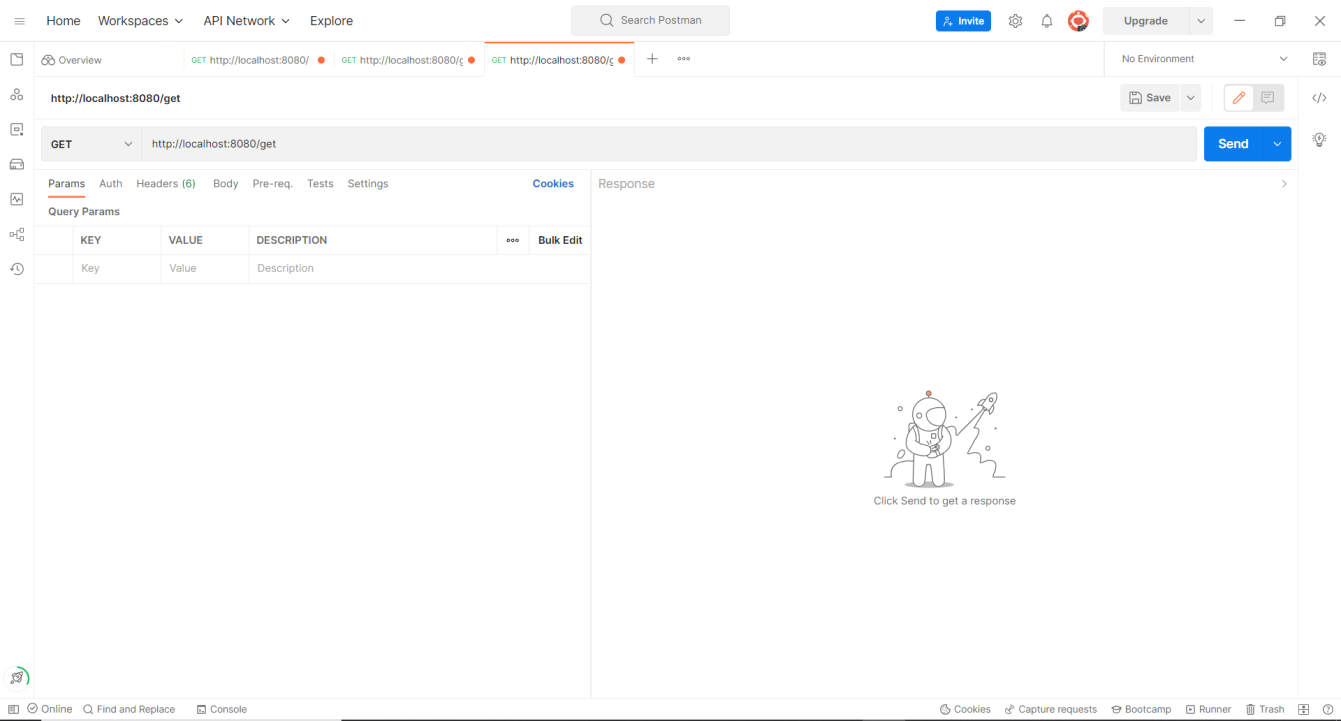
\includegraphics[scale=1]{images/Postman.png}
\caption{Postman.}
\label{fig:Postman}
\end{figure}
\newpage

\subsection{PgAdmin}

A PgAdmin\cite{PgAdmin} egy grafikus felhasználói felület a PostgreSQL kezelésére, ami a lehető legjobb megoldás lehet. Legújabb verziója a PgAdmin 4, jQuerry, JavaScript és Python kombinációjával készült. Előnyei:

\begin{itemize}
\item Kompatibilis Windows, linux és Mac operációs rendszerekkel is.
\item Bárhova telepíthető ahol PostgreSQL-t használ.
\item Van olyan lekérdező eszközei, amivel gyorsabb az adatbevitel és a hibakezelés
\end{itemize}

Rengeteg dokumentáció megtalálható hozzá amivel könnyedén el lehet kezdeni a használatát.

\begin{figure}[h]
\centering
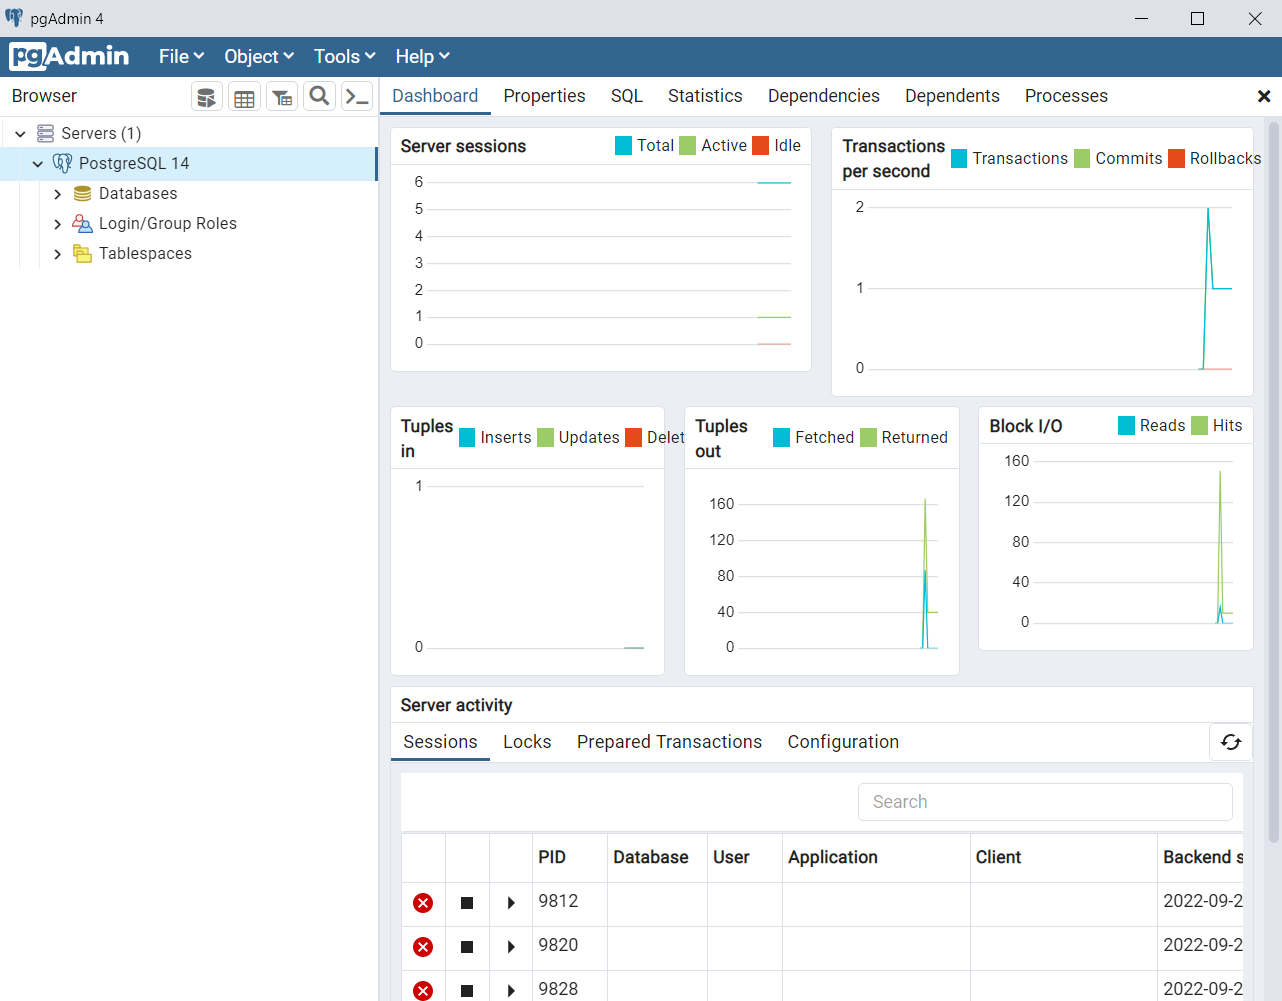
\includegraphics[scale=0.5]{images/PgAdmin.png}
\caption{PgAdmin 4.}
\label{fig:PgAdmin 4}
\end{figure}
\newpage

